
\section{Spannungsmessung}

Die elektrische Spannung $U$ ist definiert als das Verhältnis zwischen der Energie $E$ und der Ladung $Q$.
Sie gibt an, wie viel elektrische Energie umgewandelt wird, wenn eine Ladungseinheit geflossen ist.
Die Einheit der Spannung ist das Volt ($\unit{\volt}$).

\begin{greenbox}
\textbf{Spannung $U$}
$$
    U = \frac{E}{Q} \quad,\quad \left[ U \, \right] = \frac{\unit{\joule}}{\unit{\coulomb}} = \unit{\volt} \quad \text{(Volt)}
$$
\end{greenbox}

\begin{figure}[h!]
    \centering
    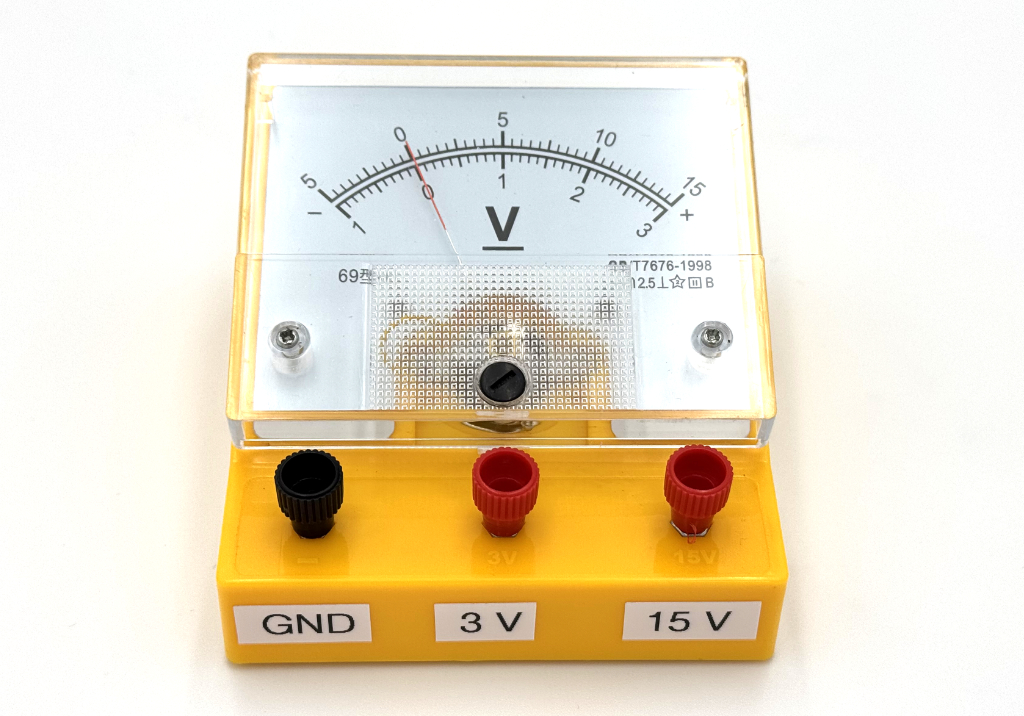
\includegraphics[width=8cm]{_images/volt_meter}
    \caption{Spannungsmessgerät, auch Voltmeter genannt.}
    \label{fig:voltmeter}
\end{figure}

Das Voltmeter ist ein Instrument, das die Spannung zwischen zwei Punkten in einem
elektrischen Kreis messen kann.

\begin{greenbox}
Spannungsmessgeräte werden immer parallel zum Verbraucher angeschlossen.
\end{greenbox}




\exercise{Korrekte Spannungsmessung}

Gib bei den folgenden Schaltplänen an, wo das Voltmeter richtig oder falsch angeschlossen ist.

% Raster für die Antworten
\begin{tikzpicture}
    \draw[step=4mm,gray,very thin] (0,0) grid (14.8,-6.41);

    \node at (1,-0.6) {a)};
    \node  at (3.5,-3)
        {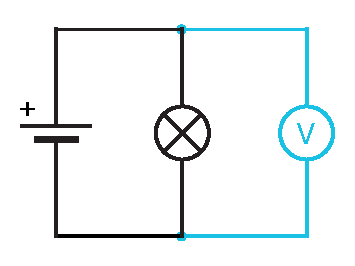
\includegraphics[width=6cm]{_images/volt_messung_1.pdf}};

    \node at (8,-0.6) {b)};
    \node  at (10.5,-3)
        {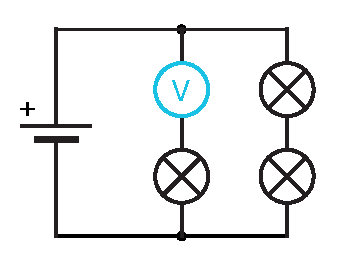
\includegraphics[width=6cm]{_images/volt_messung_2.pdf}};

    \answer{
        \draw (1.4,-0.2) node[anchor=north west,align=left,text width=13cm] {%
      		\marker%
        korrekt
        };
        \draw (1.4,-5) node[anchor=north west,align=left,text width=13cm] {%
      		\marker%
        Parallel zum Verbraucher\\
        ist korrekt.
        };


        \draw (8.4,-0.2) node[anchor=north west,align=left,text width=13cm] {%
      		\marker%
        falsch
        };
        \draw (8.4,-5) node[anchor=north west,align=left,text width=13cm] {%
      		\marker%
            In Serie zum Verbraucher\\
            ist falsch.
        };
    }
\end{tikzpicture}





\newpage
\experiment{Spannungsmessung}


Baue das Experiment aus siehe \fref{fig:voltage_measurement} auf.

\begin{figure}[h!]
    \centering
    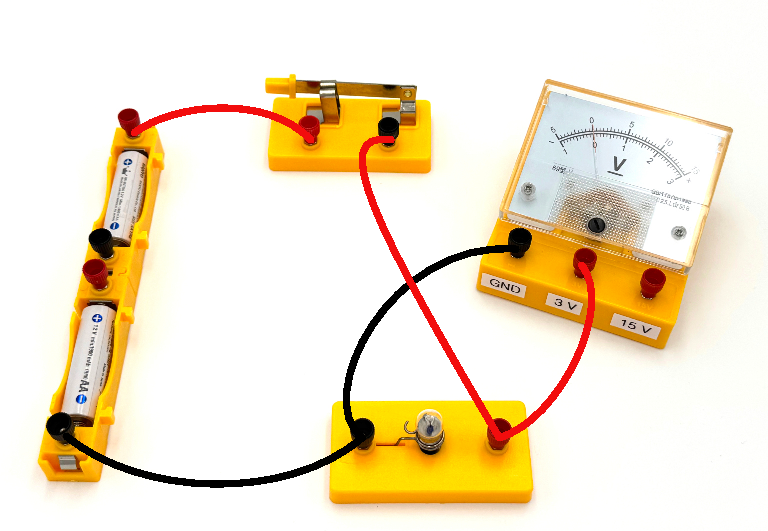
\includegraphics[width=9cm]{_images/volt_setup.pdf}
    \caption{Spannungsmessung}
    \label{fig:voltage_measurement}
\end{figure}

Schliesse den Schalter und notiere deine Beobachtungen. Beantworte die folgenden Fragen:

\begin{enumerate}
    \item Miss die Spannung mit dem Voltmeter (3 V).
    \item Miss die Spannung mit dem Voltmeter (15 A).
    \item Vertausche die beiden Kabel beim Voltmeter.
    \item Vervollständige den Schaltplan.
\end{enumerate}


% Raster für die Antworten
\begin{tikzpicture}
    \draw[step=4mm,gray,very thin] (0,0) grid (14.8,-8.4);

    \noanswer{
        \node  at (7,-6)
            {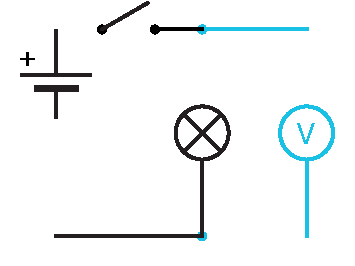
\includegraphics[width=6cm]{_images/volt_setup_schaltplan.pdf}};
    }

    \answer{
        \node  at (7,-6)
            {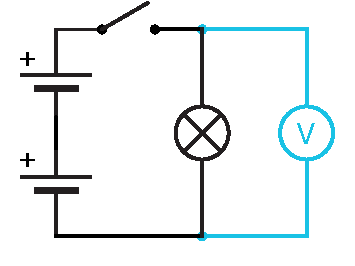
\includegraphics[width=6cm]{_images/volt_setup_schaltplan_loesung.pdf}};
    }

    \answer{
        \draw (0.3,0.14) node[anchor=north west,align=left,text width=13cm] {%
      		\marker%

            \textbf{1.} Die Spannung beträgt ca. 2.4 V. \\
            \textbf{2.} Der Ausschlag der Nadel ist beim 15 V-Bereich kleiner. Die Spannung beträgt aber immer noch ca. 2.4 V.\\
            \textbf{3.} Die Nadel schlägt in die negative Richtung aus.\\

        };
    }
\end{tikzpicture}





\newpage
\experiment{Spannung in der Serienschaltung}

In diesem Experiment soll untersucht werden, wie gross die Spannungen in einer Serienschaltung sind.
Das Voltmeter wird dazu nacheinander an verschiedenen Stellen im Stromkreis platziert.

\begin{figure}[h!]
\centering
    \begin{subfigure}[b]{0.305\textwidth}
    \centering
    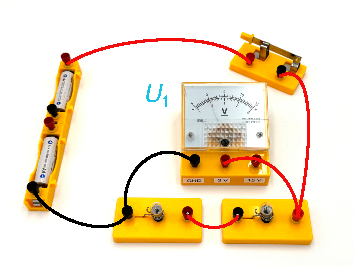
\includegraphics[width=4.6cm]{_images/volt_serie_1.pdf}
    \end{subfigure}
\quad
    \begin{subfigure}[b]{0.305\textwidth}
    \centering
    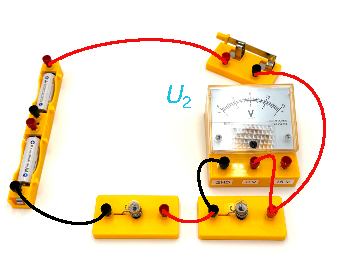
\includegraphics[width=4.6cm]{_images/volt_serie_2.pdf}
    \end{subfigure}
\quad
    \begin{subfigure}[b]{0.305\textwidth}
    \centering
    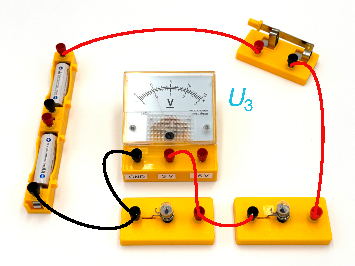
\includegraphics[width=4.6cm]{_images/volt_serie_3.pdf}
    \end{subfigure}
\end{figure}


% Raster für die Antworten
\begin{tikzpicture}
    \draw[step=4mm,gray,very thin] (0,0) grid (14.8,-16);

    \node  at (3.5,-3.5)
        {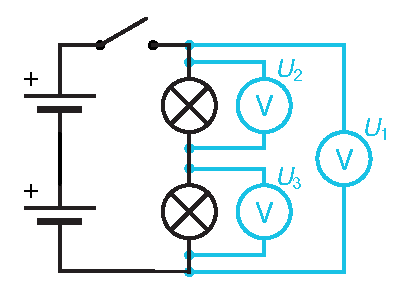
\includegraphics[width=7cm]{_images/volt_serie}};

        \draw (8,-1.85) node[anchor=north west,align=left,text width=13cm] {%
      		\marker%

            U$_{\text{1}}$ = \answer{2.4 V}  \\
            U$_{\text{2}}$ = \answer{1.2 V} \\
            U$_{\text{3}}$ = \answer{1.2 V}  \\

        };

        \draw (1,-6.6) node[anchor=north west,align=left,text width=12cm] {%
      		\marker%

            Fazit\\
            \answer{Die Spannung U$_{\text{1}}$ über beiden Lampen zusammen ist die Summe aus den
            Spannungen U$_{\text{2}}$ und U$_{\text{3}}$ über den einzelnen Lampen.}

        };
\end{tikzpicture}



\newpage
\experiment{Spannungsmessung in der Parallelschaltung}

In diesem Experiment werden die Spannungen in einer Parallelschaltung untersucht.
Dazu werden die Spannungen über die einzelnen Lampen gemessen.

\begin{figure}[h!]
\centering
    \begin{subfigure}[b]{0.305\textwidth}
    \centering
    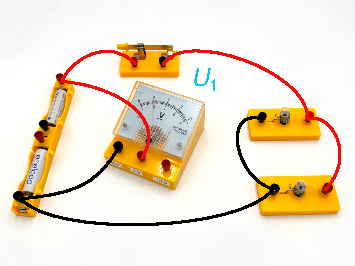
\includegraphics[width=4.6cm]{_images/volt_parallel_1.pdf}
    \end{subfigure}
\quad
    \begin{subfigure}[b]{0.305\textwidth}
    \centering
    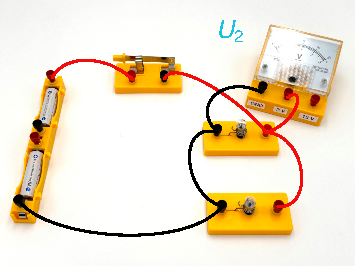
\includegraphics[width=4.6cm]{_images/volt_parallel_2.pdf}
    \end{subfigure}
\quad
        \begin{subfigure}[b]{0.305\textwidth}
        \centering
        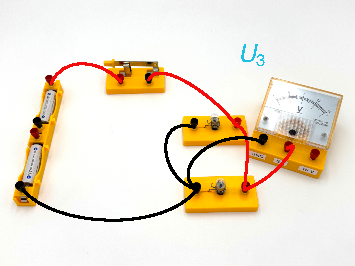
\includegraphics[width=4.6cm]{_images/volt_parallel_3.pdf}
        \end{subfigure}
\end{figure}


% Raster für die Antworten
\begin{tikzpicture}
    \draw[step=4mm,gray,very thin] (0,0) grid (14.8,-14);

    \node  at (4,-3.5)
        {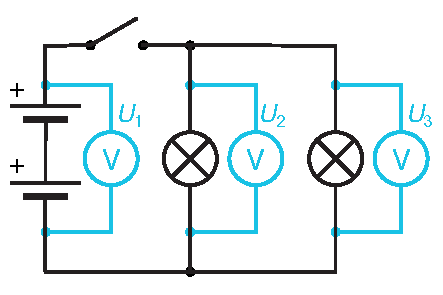
\includegraphics[width=8cm]{_images/volt_parallel}};

        \draw (9,-1.85) node[anchor=north west,align=left,text width=13cm] {%
      		\marker%

            U$_{\text{1}}$ = \answer{2.4 V}  \\
            U$_{\text{2}}$ = \answer{2.4 V} \\
            U$_{\text{3}}$ = \answer{2.4 V} \\

        };

        \draw (1,-6.6) node[anchor=north west,align=left,text width=12cm] {%
      		\marker%

            Fazit\\
            \answer{Bei der Parallelschaltung sind die Spannungen U$_{\text{2}}$ und U$_{\text{3}}$ über den beiden Lampen gleich gross, wie die Spannung U$_{\text{1}}$ der Batterie.}

        };
\end{tikzpicture}
